\subsection{Giao diện quản lý process portfolio của workspace}

\begin{figure}[H]
    \centering
    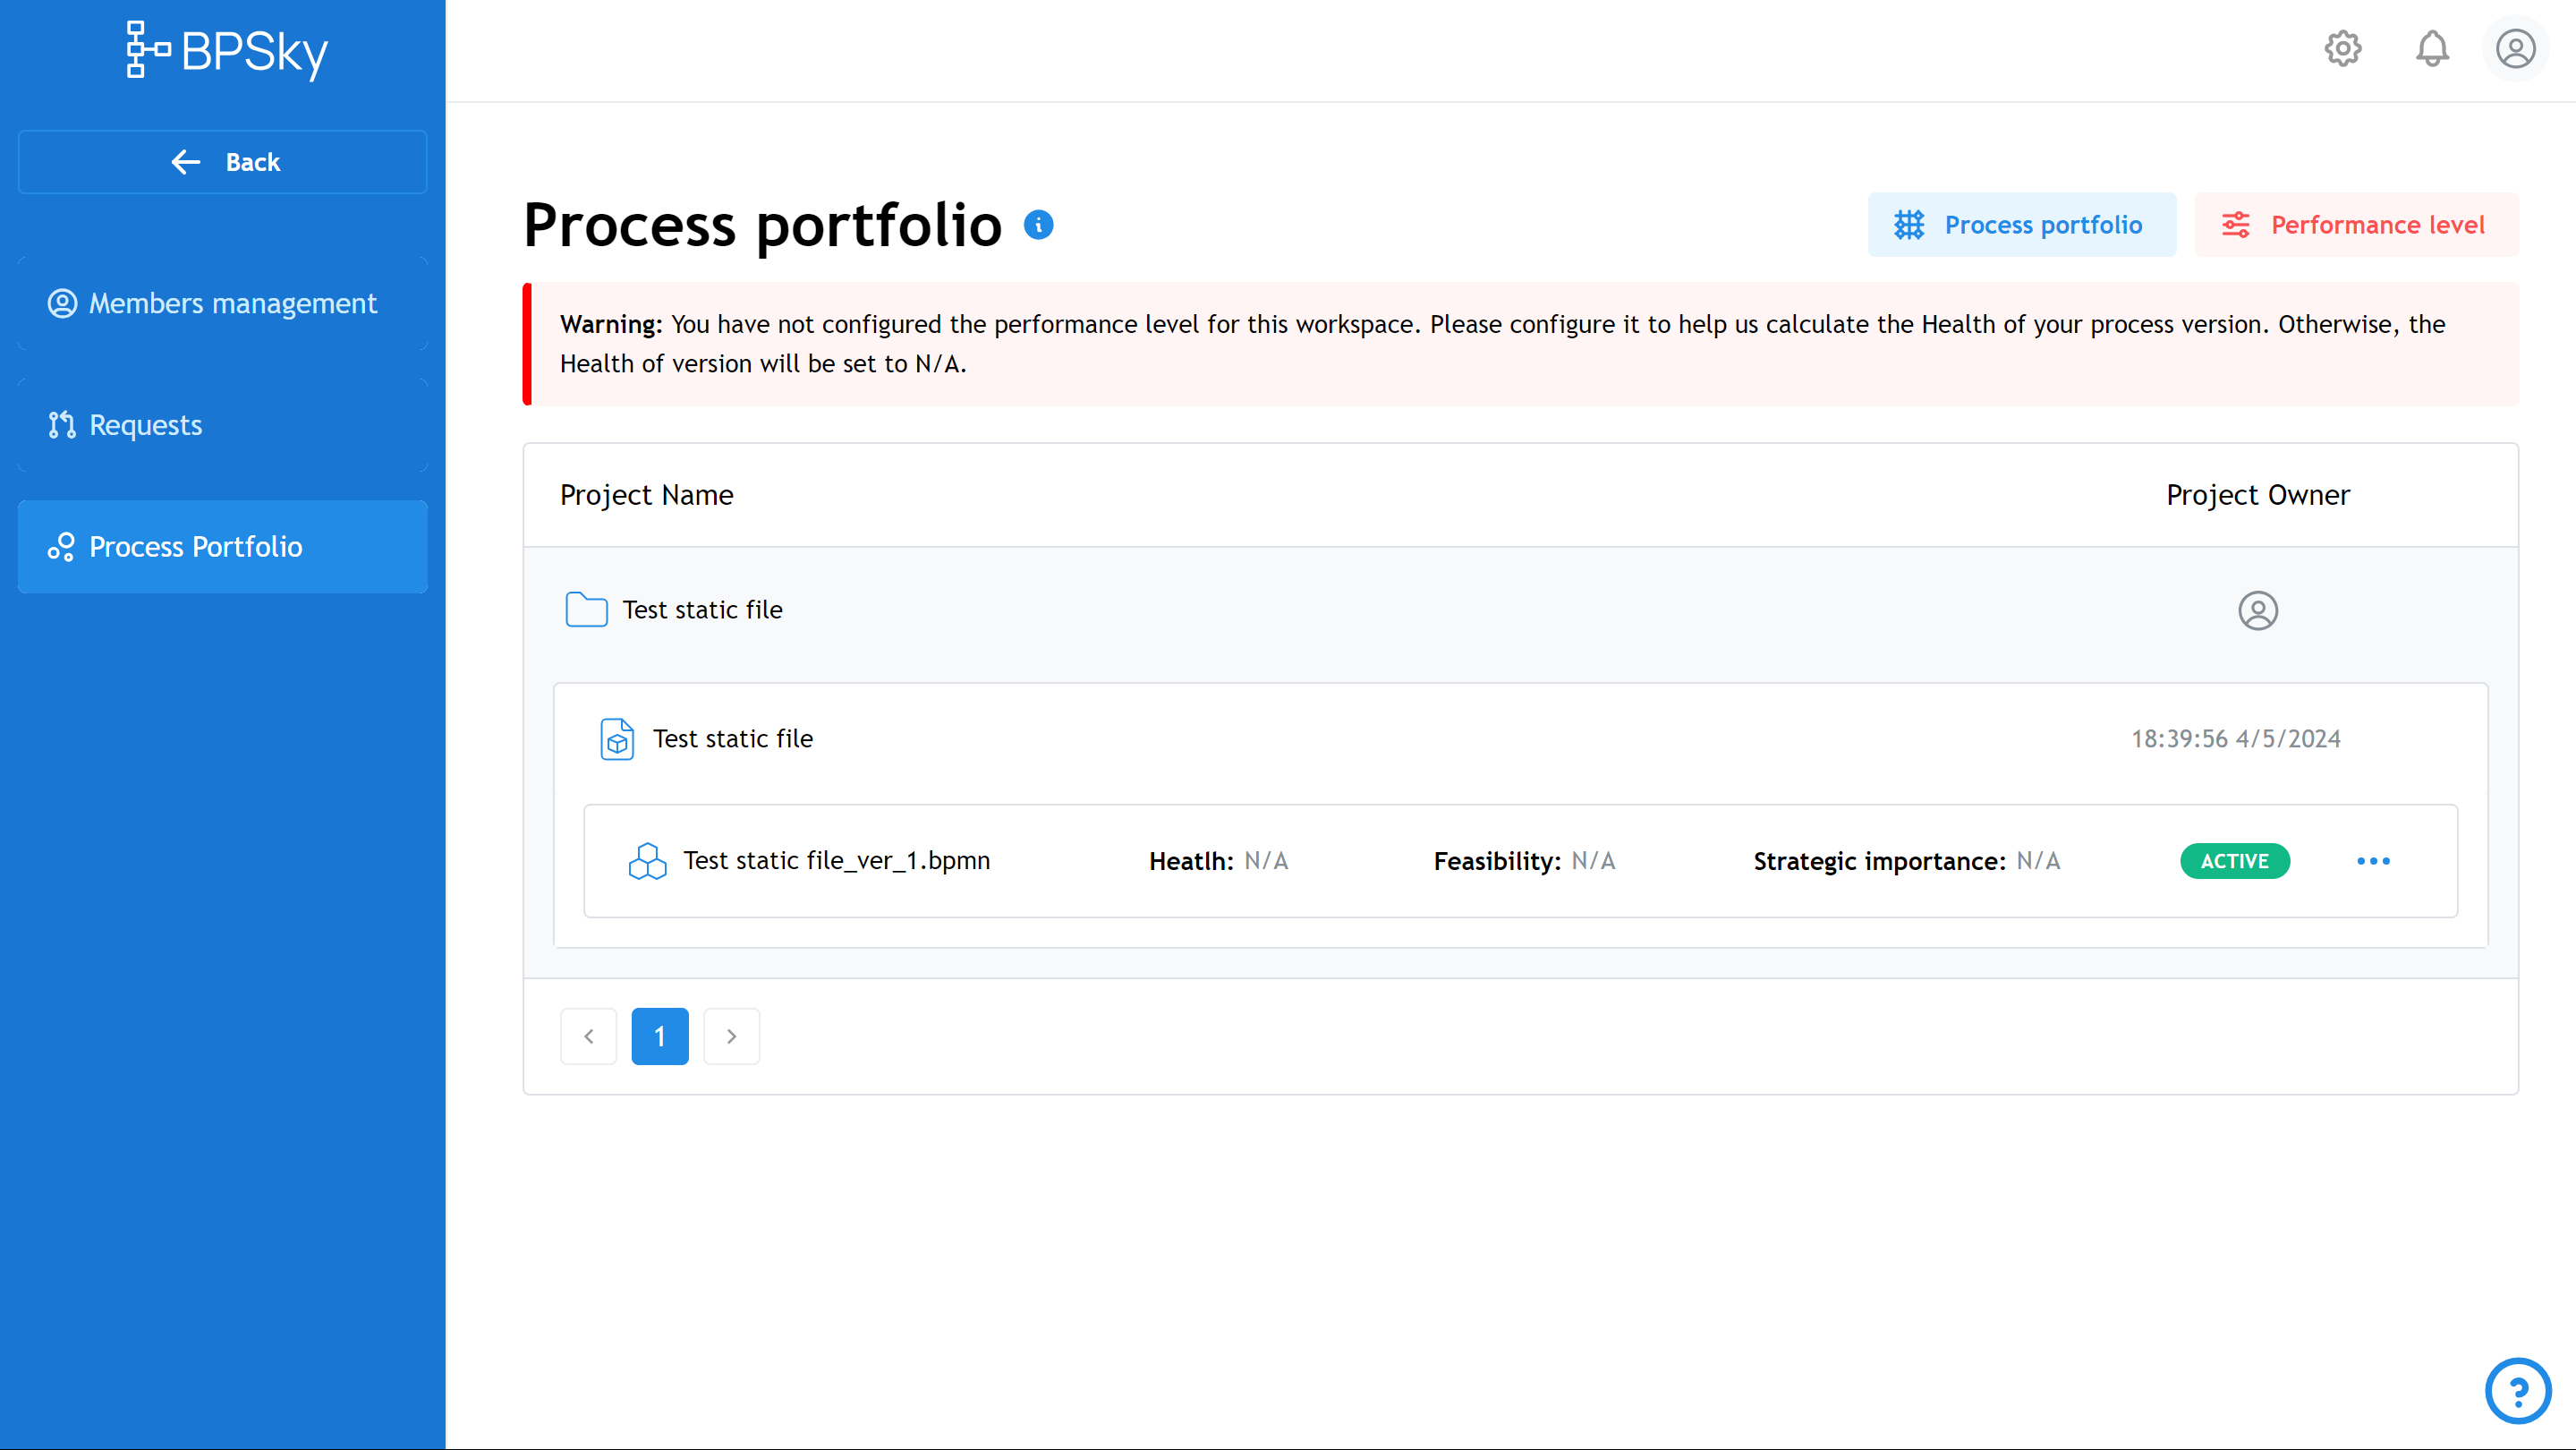
\includegraphics[ width = 0.8\linewidth]{Content/Hiện thực hệ thống/documents/Hiện thực giao diện người dùng/images/ProcessPortfolio.png}
    \vspace{0.5cm}
    \caption{Giao diện quản lý process portfolio của workspace}
    \label{fig: Giao diện quản lý process portfolio của workspace}
\end{figure}

Sau khi người dùng chọn Process portfolio trên thanh điều hướng, hệ thống sẽ chuyển hướng người dùng tới trang quản lý/khởi tạo process portfolio cho workspace. Người dùng có thể thấy được danh sách những process version/project có trong workspace. Người dùng có thể chọn nút Process portfolio để xem biểu đồ process portfolio của workspace hoặc nút Performance level để chỉnh sửa các thông tin liên quan tới thang đo được sử dụng chung cho toàn bộ workspace.

\begin{figure}[H]
    \centering
    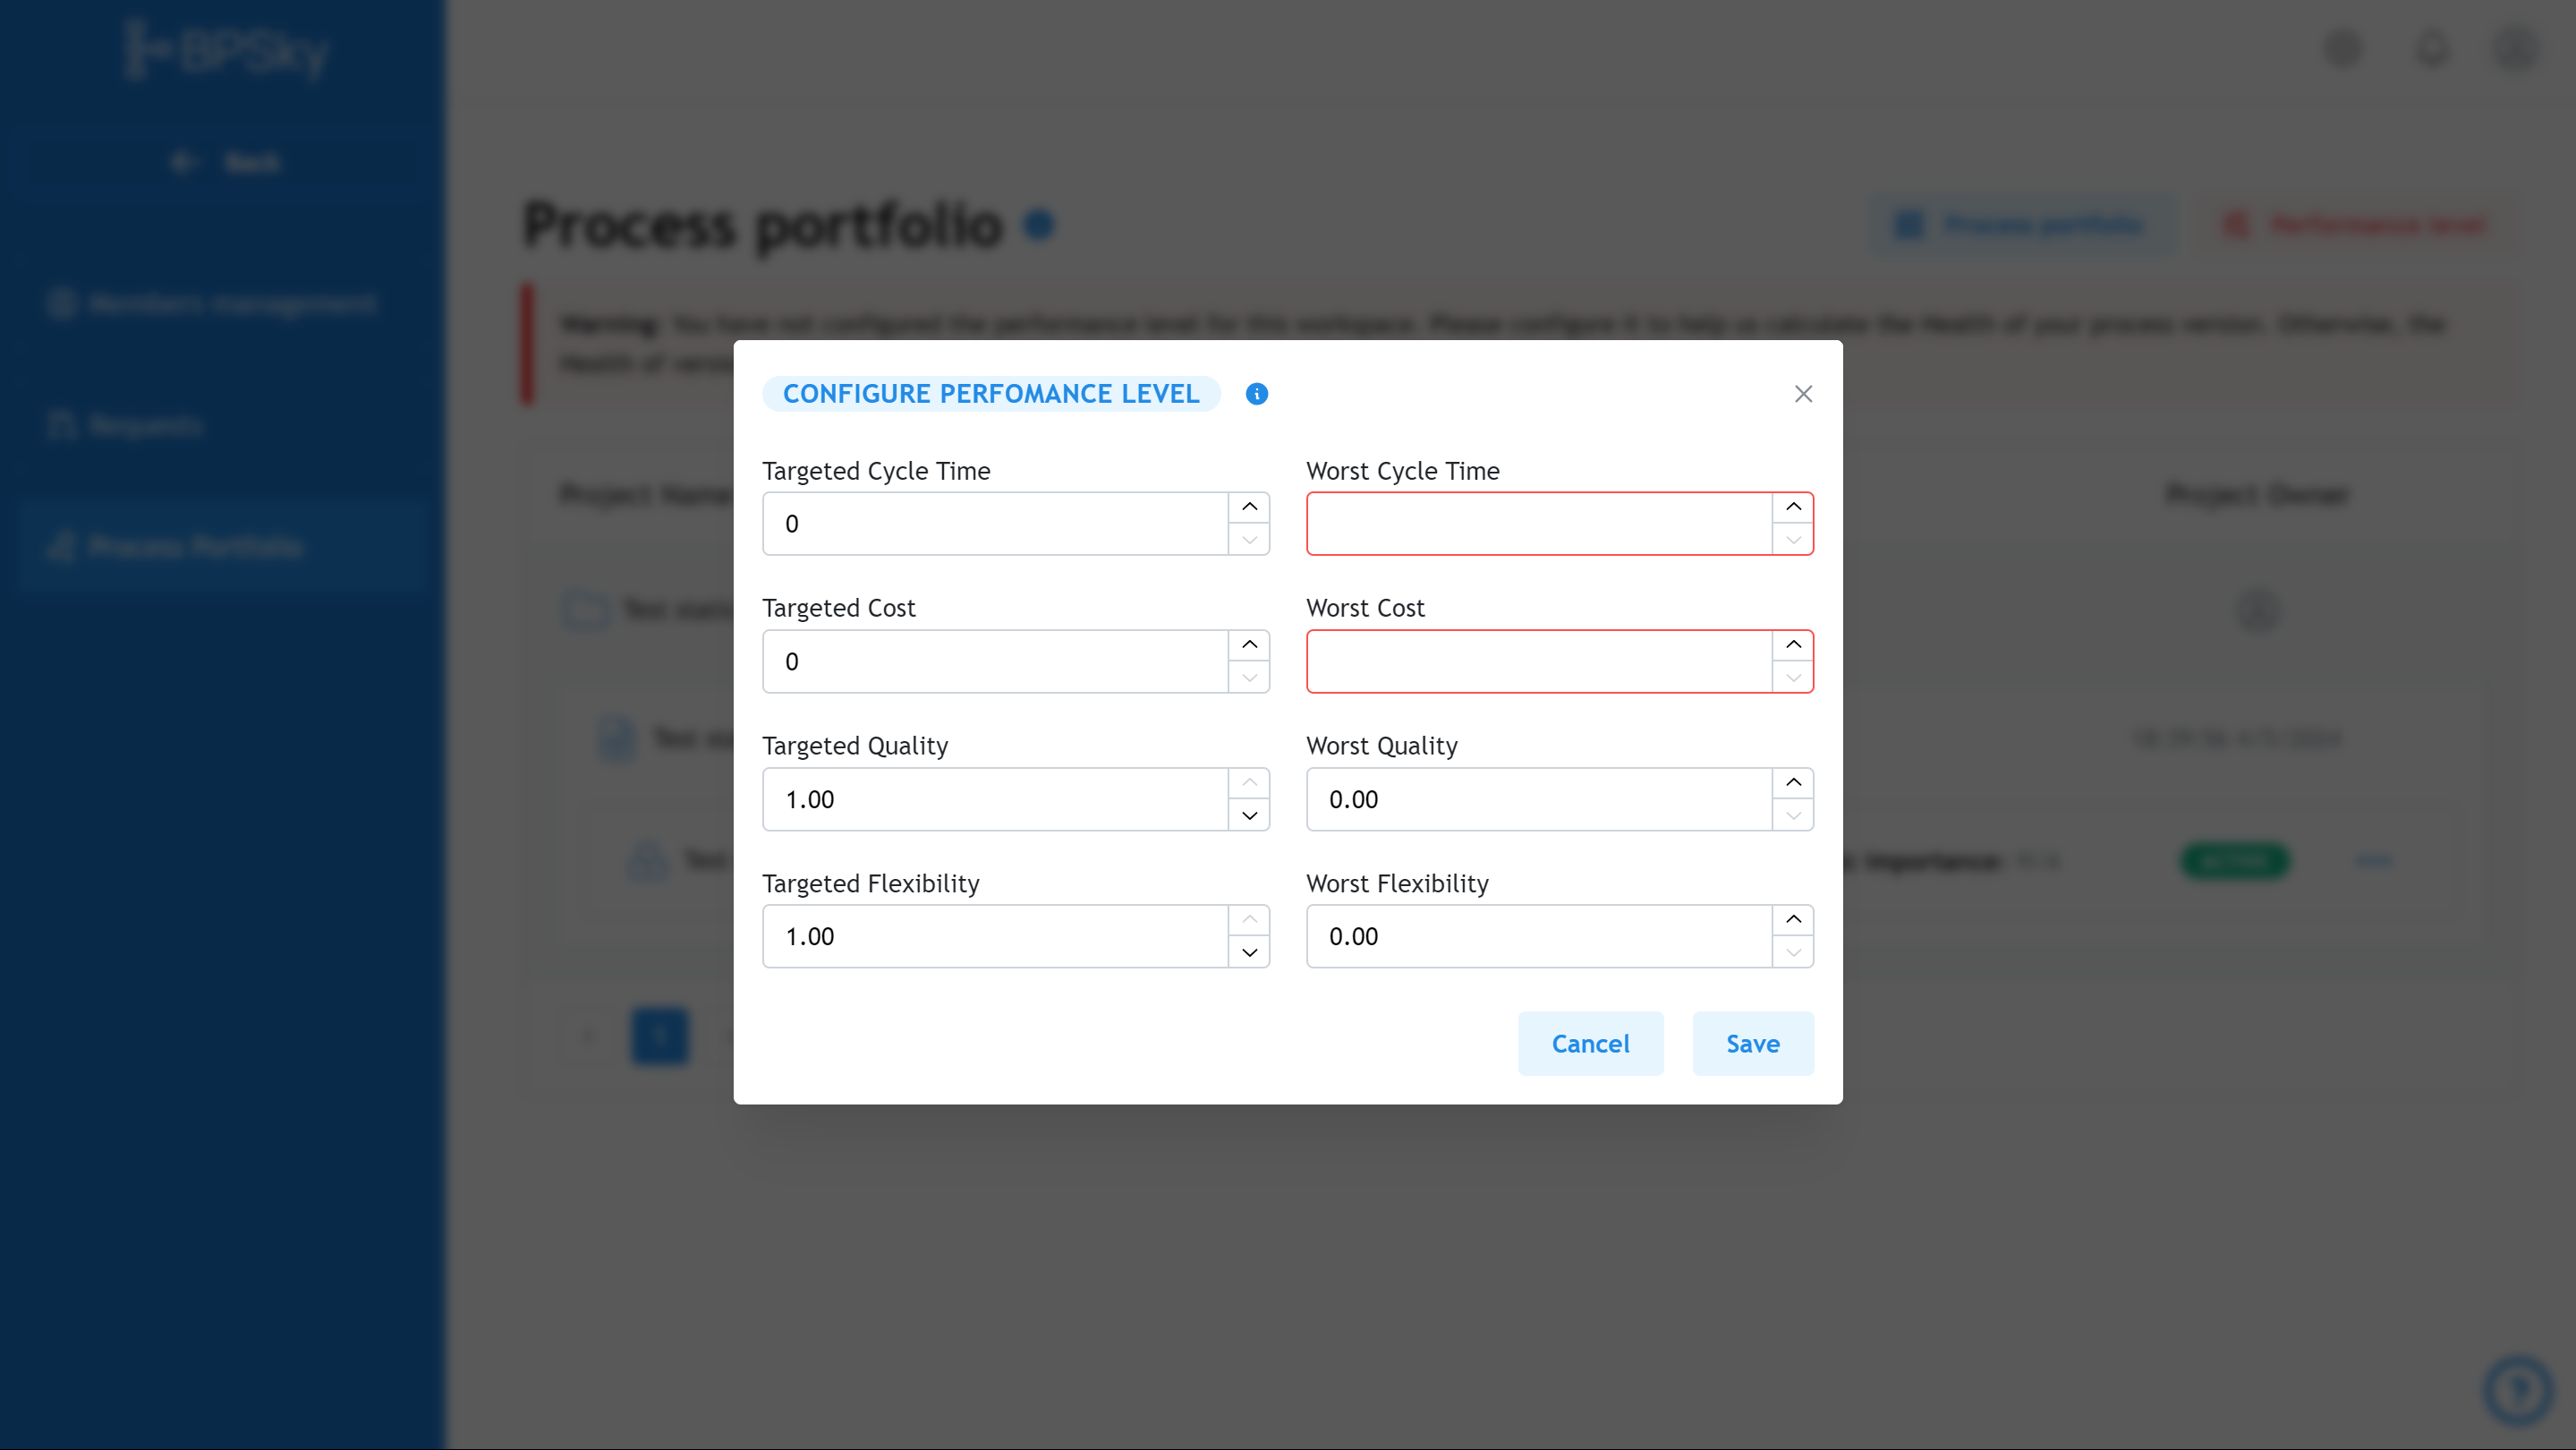
\includegraphics[ width = 0.8\linewidth]{Content/Hiện thực hệ thống/documents/Hiện thực giao diện người dùng/images/WorkspaceMeasurement.png}
    \vspace{0.5cm}
    \caption{Giao diện chỉnh sửa giá trị thang đo cho process portfolio của workspace}
    \label{fig: Giao diện chỉnh sửa giá trị thang đo cho process portfolio của workspace}
\end{figure}

Người dùng sẽ được yêu cầu nhập thông tin liên quan tới thang đo cho process portfolio của workspace. Sau khi nhập thông tin, người dùng có thể chọn nút Save để lưu thông tin hoặc nút Cancel để hủy bỏ thao tác. Thông tin này sẽ được sử dụng để xác định thang đo (giá trị lớn nhất, giá trị nhỏ nhất) khi tính toán những thông số liên quan tới hiệu suất của process version (Heatlh).

\begin{figure}[H]
    \centering
    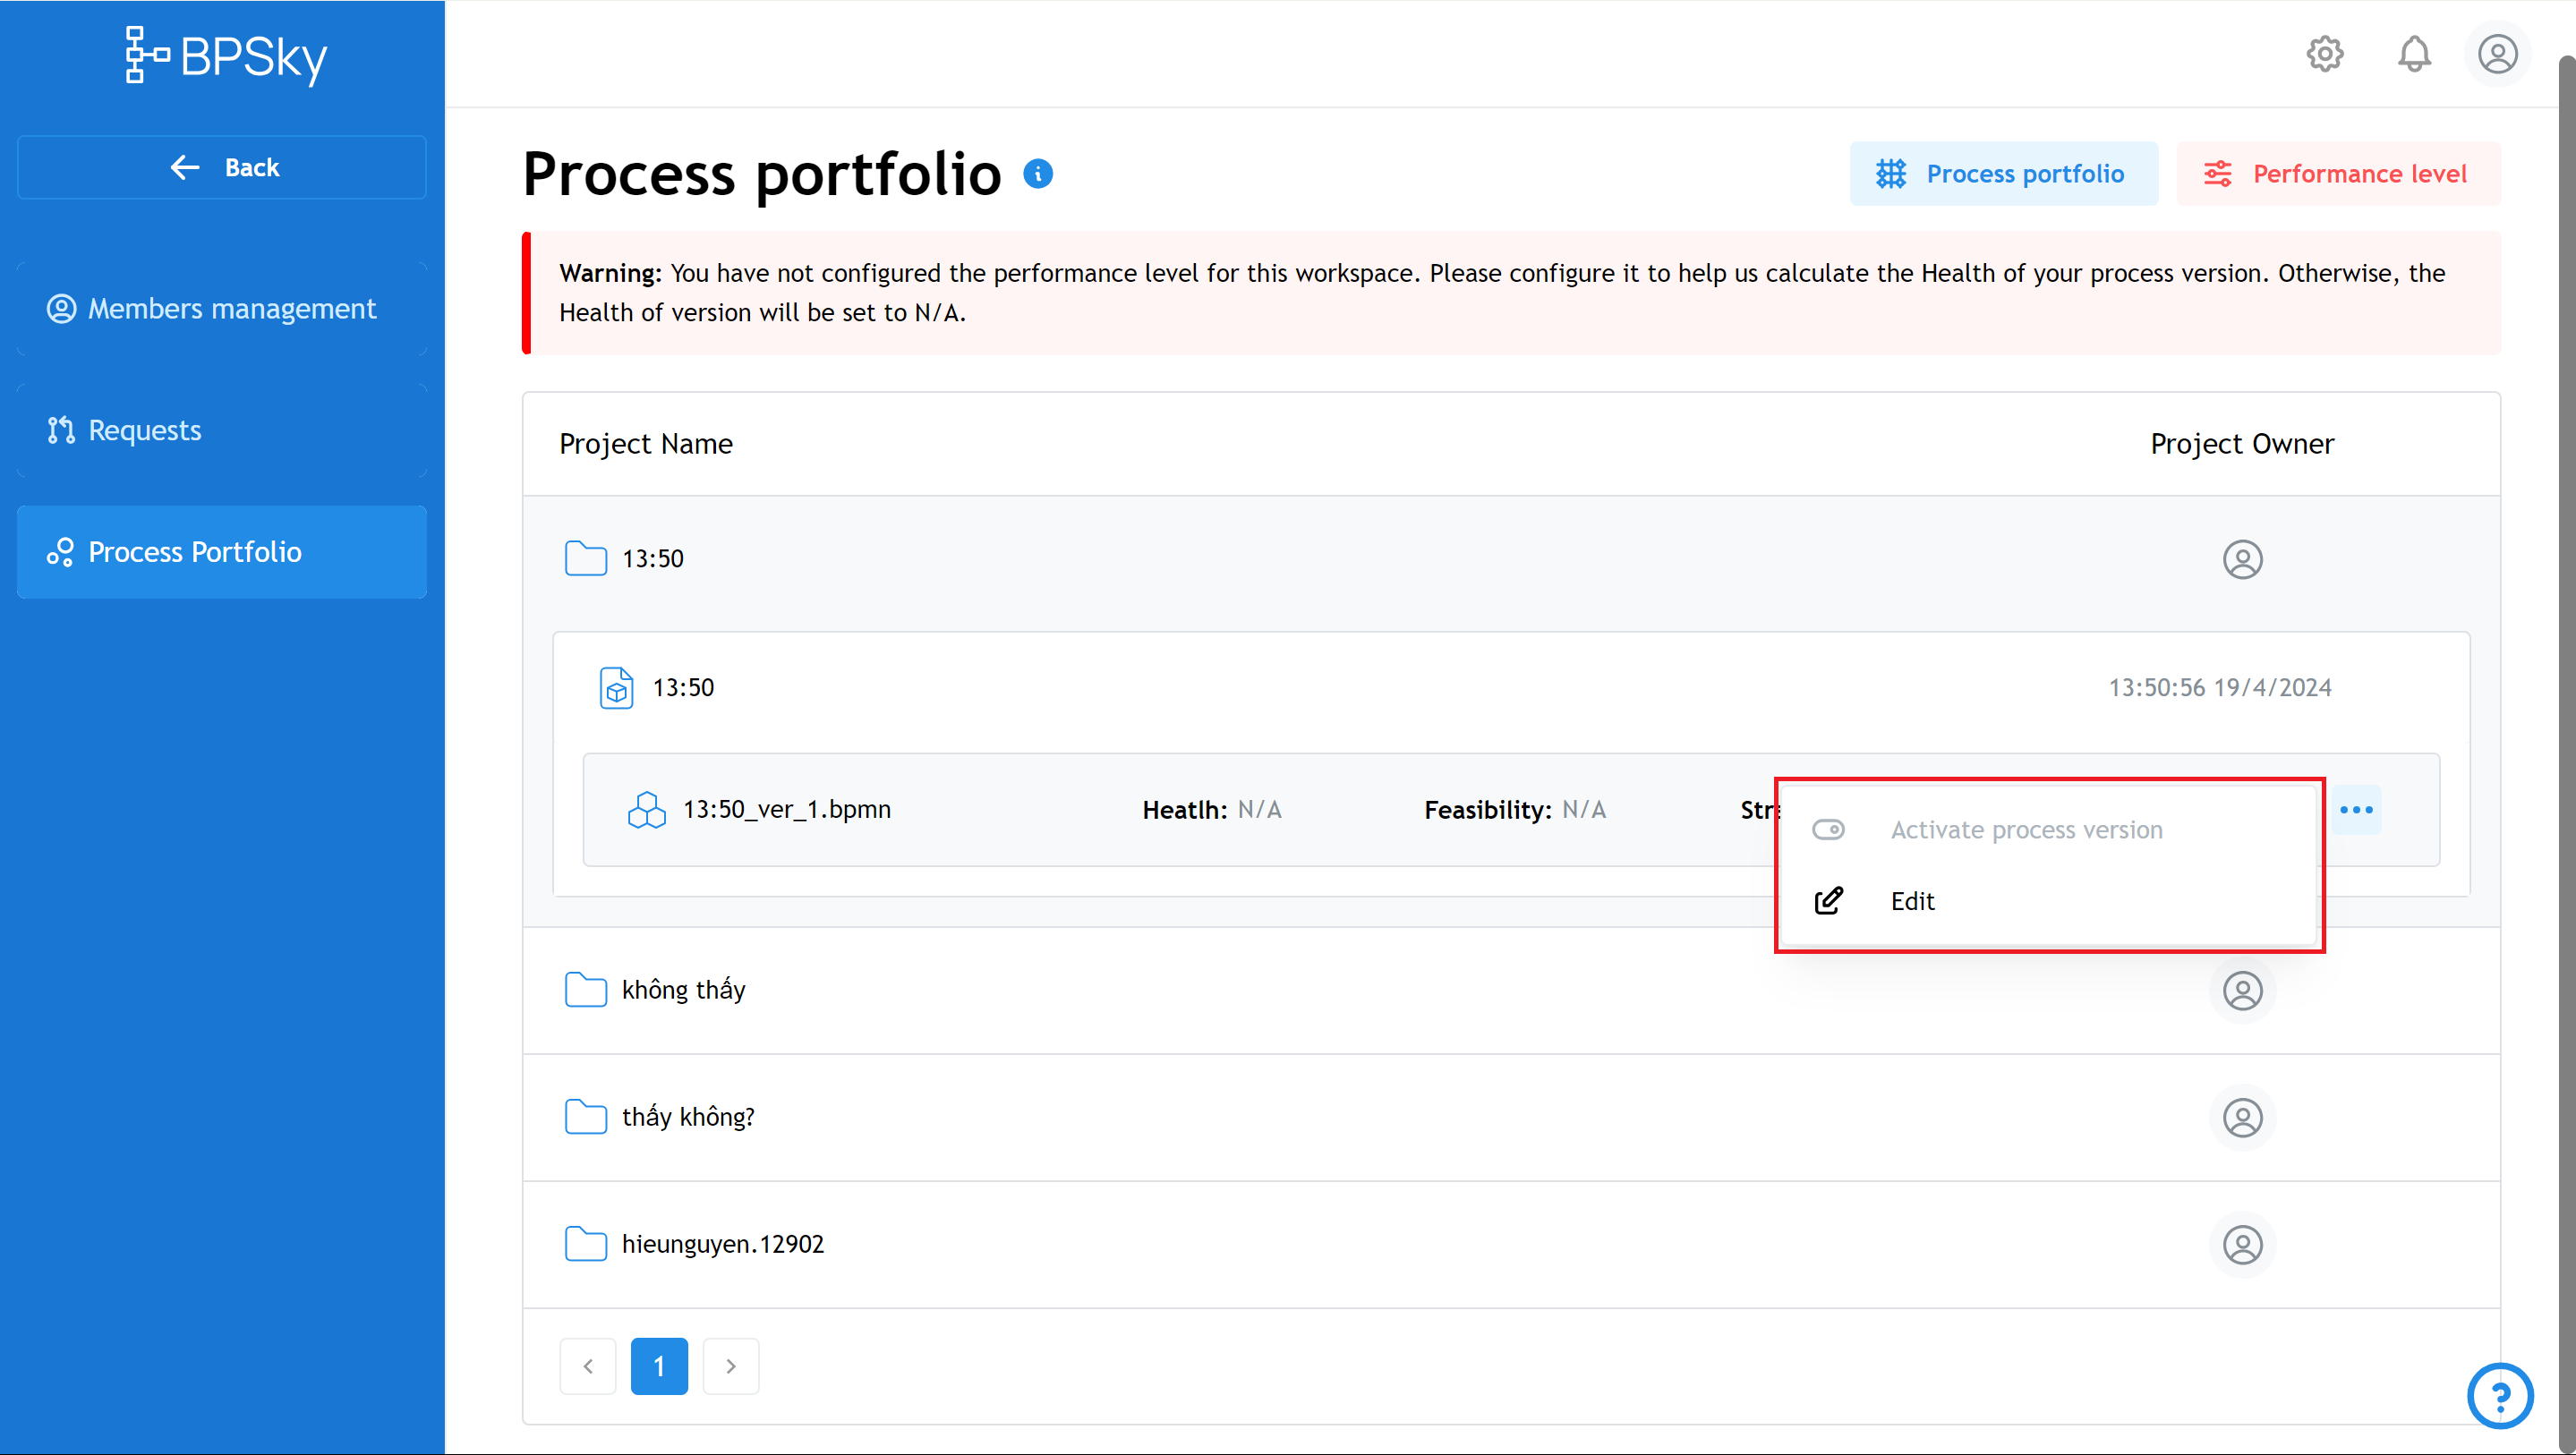
\includegraphics[ width = 0.8\linewidth]{Content/Hiện thực hệ thống/documents/Hiện thực giao diện người dùng/images/ProcessVersionEdit.png}
    \vspace{0.5cm}
    \caption{Giao diện menu của process version}
    \label{fig: Giao diện menu của process version}
\end{figure}

Người dùng có thể chọn nút Edit trong menu trên item tương ứng để chỉnh sửa thông tin liên quan tới thang đo của process version. Sau khi chỉnh sửa xong, người dùng có thể chọn nút Save để lưu thông tin hoặc nút Cancel để hủy bỏ thao tác. Hoặc chọn Activate để kích hoạt process version tương ứng, mỗi một process chỉ có một version được đặt trạng thái active. Version này sẽ được sử dụng để khởi tạo biểu đồ process portfolio.

\begin{figure}[H]
    \centering
    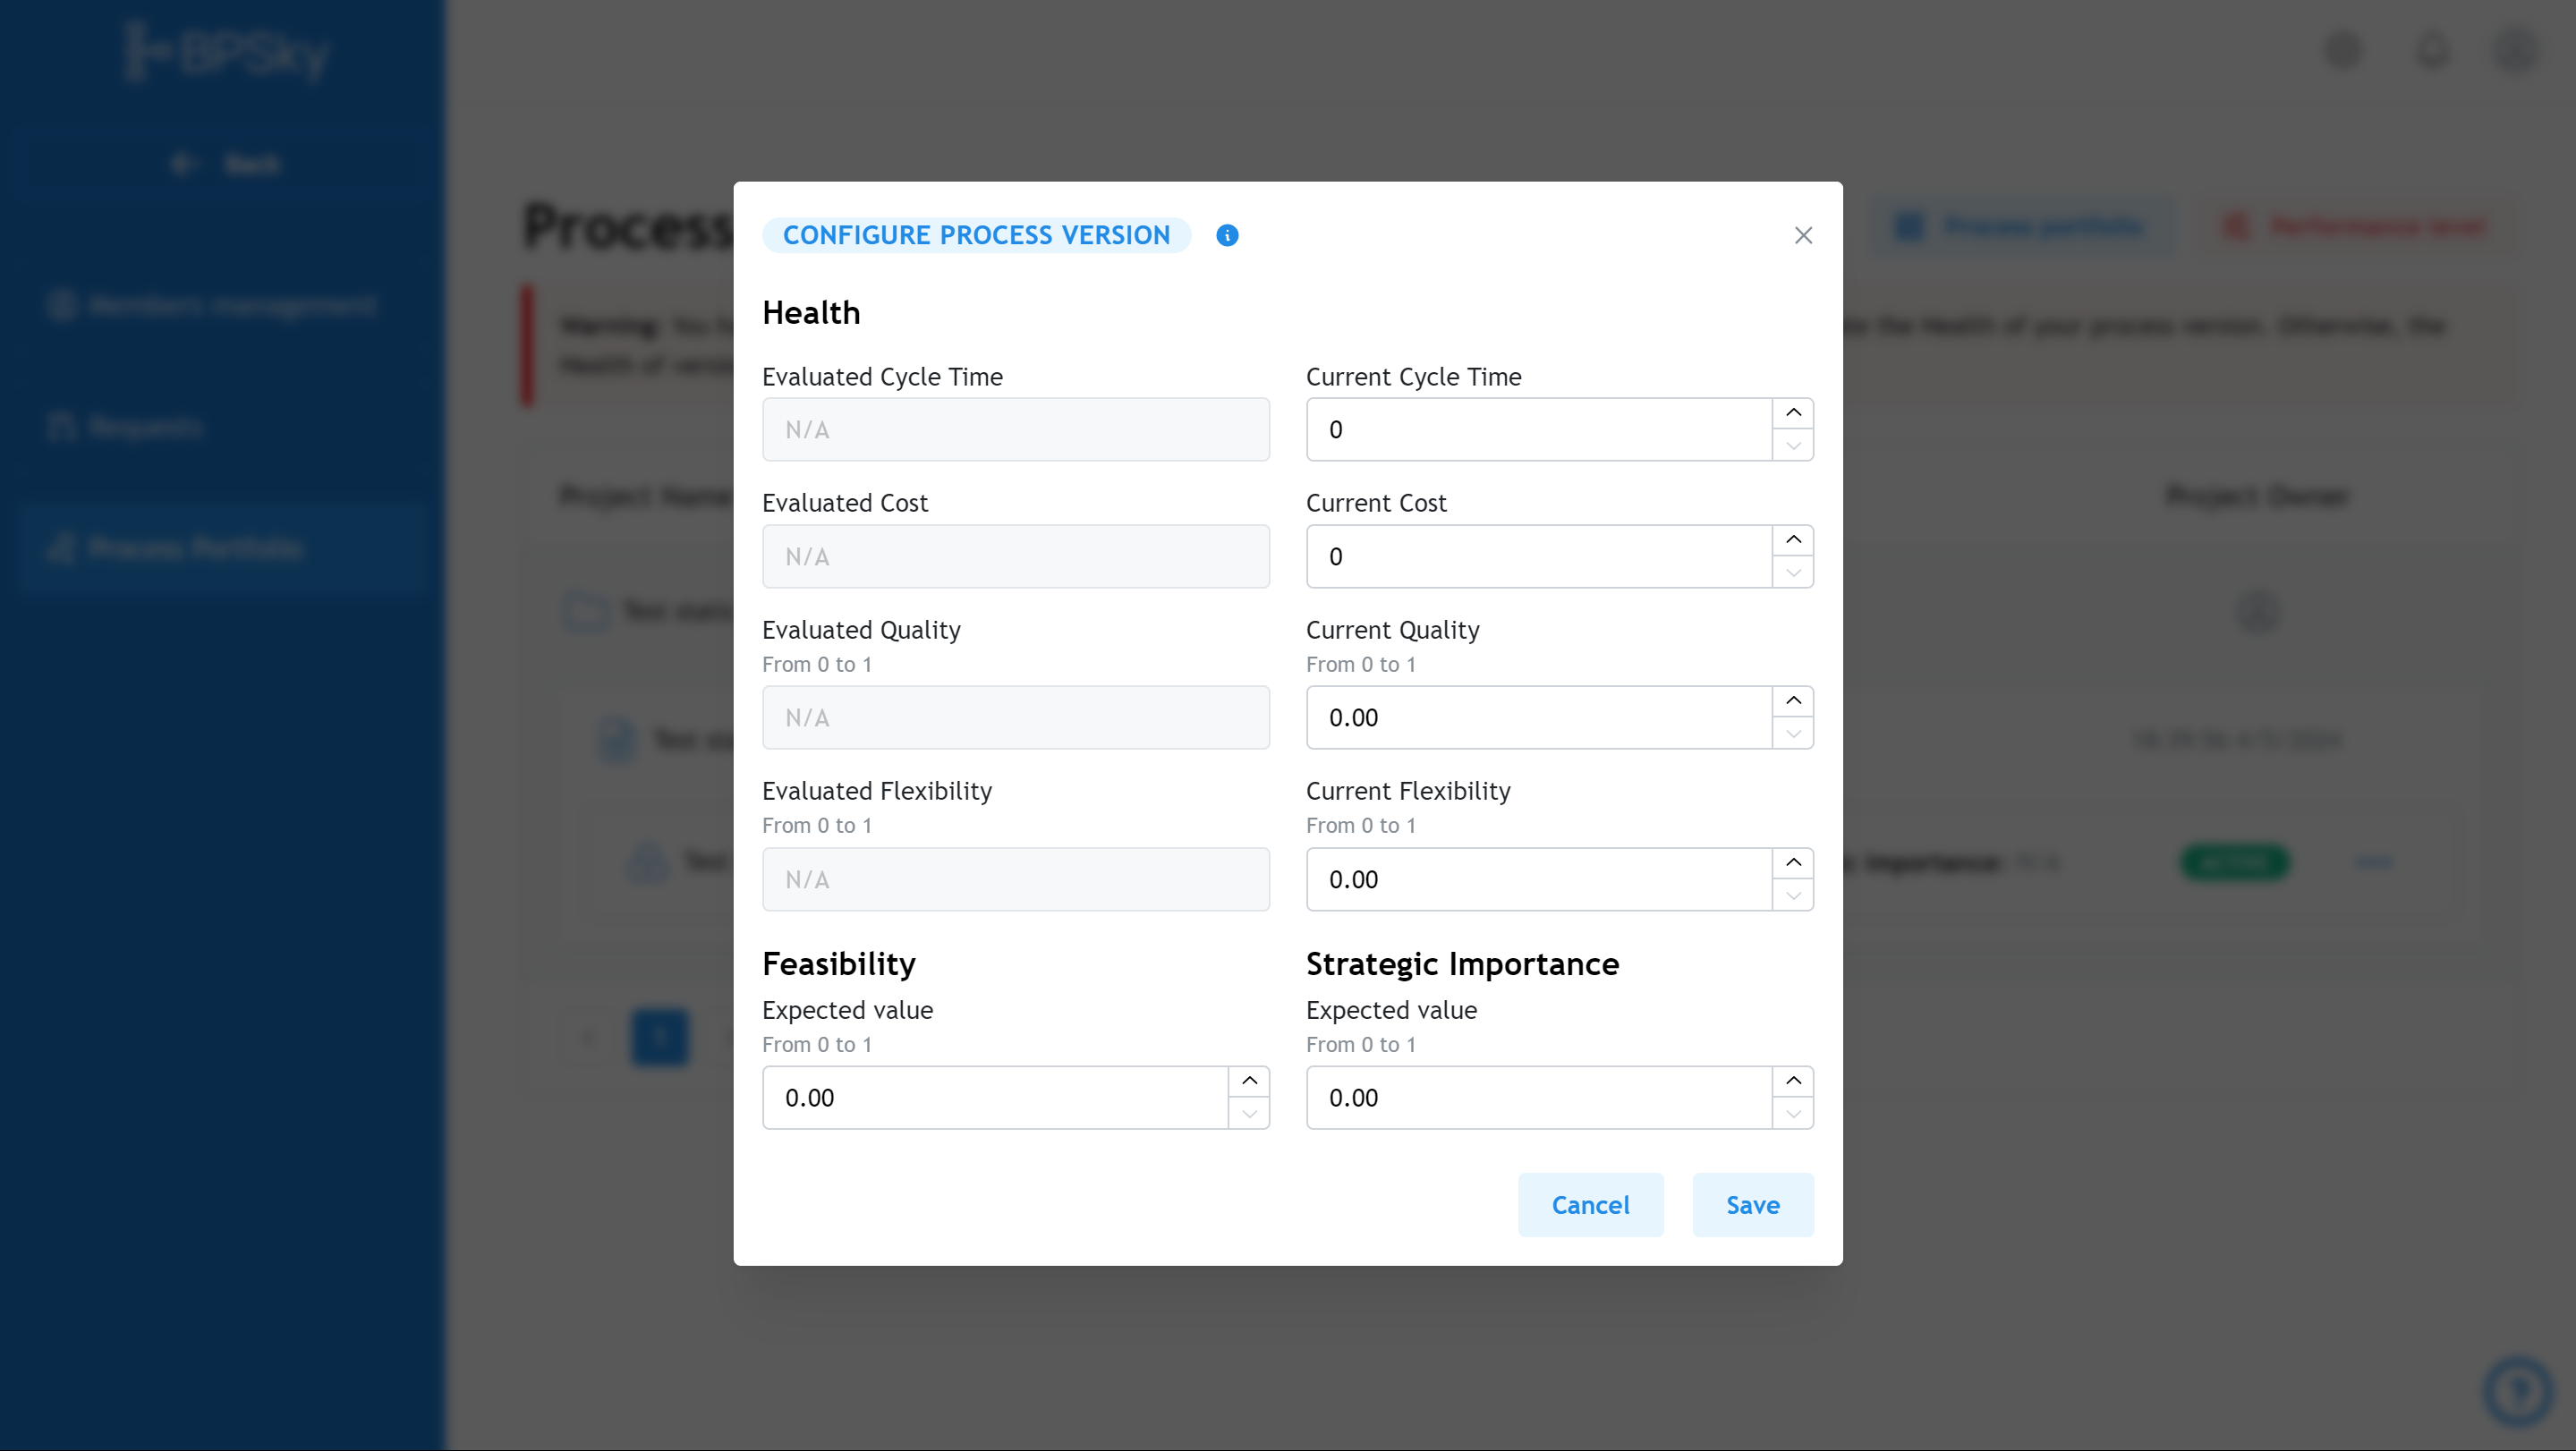
\includegraphics[ width = 0.8\linewidth]{Content/Hiện thực hệ thống/documents/Hiện thực giao diện người dùng/images/ProcessVersionMeasurement.png}
    \vspace{0.5cm}
    \caption{Giao diện chỉnh sửa giá trị của process version trong workspace}
    \label{fig: Giao diện chỉnh sửa giá trị của process version trong workspace}
\end{figure}

Nếu người dùng chọn Edit trong menu thì người dùng sẽ được yêu cầu nhập thông tin liên quan tới process version tương ứng. Hệ thống sẽ mở modal bao gồm thông tin về các giá trị Strategic importance (Mức độ quan trọng chiến lược), Feasibility (Tính khả thi) và Health (Hiệu suất) của version đó. Sau khi nhập thông tin, người dùng có thể chọn nút Save để lưu thông tin hoặc nút Cancel để hủy bỏ thao tác.

\begin{figure}[H]
    \centering
    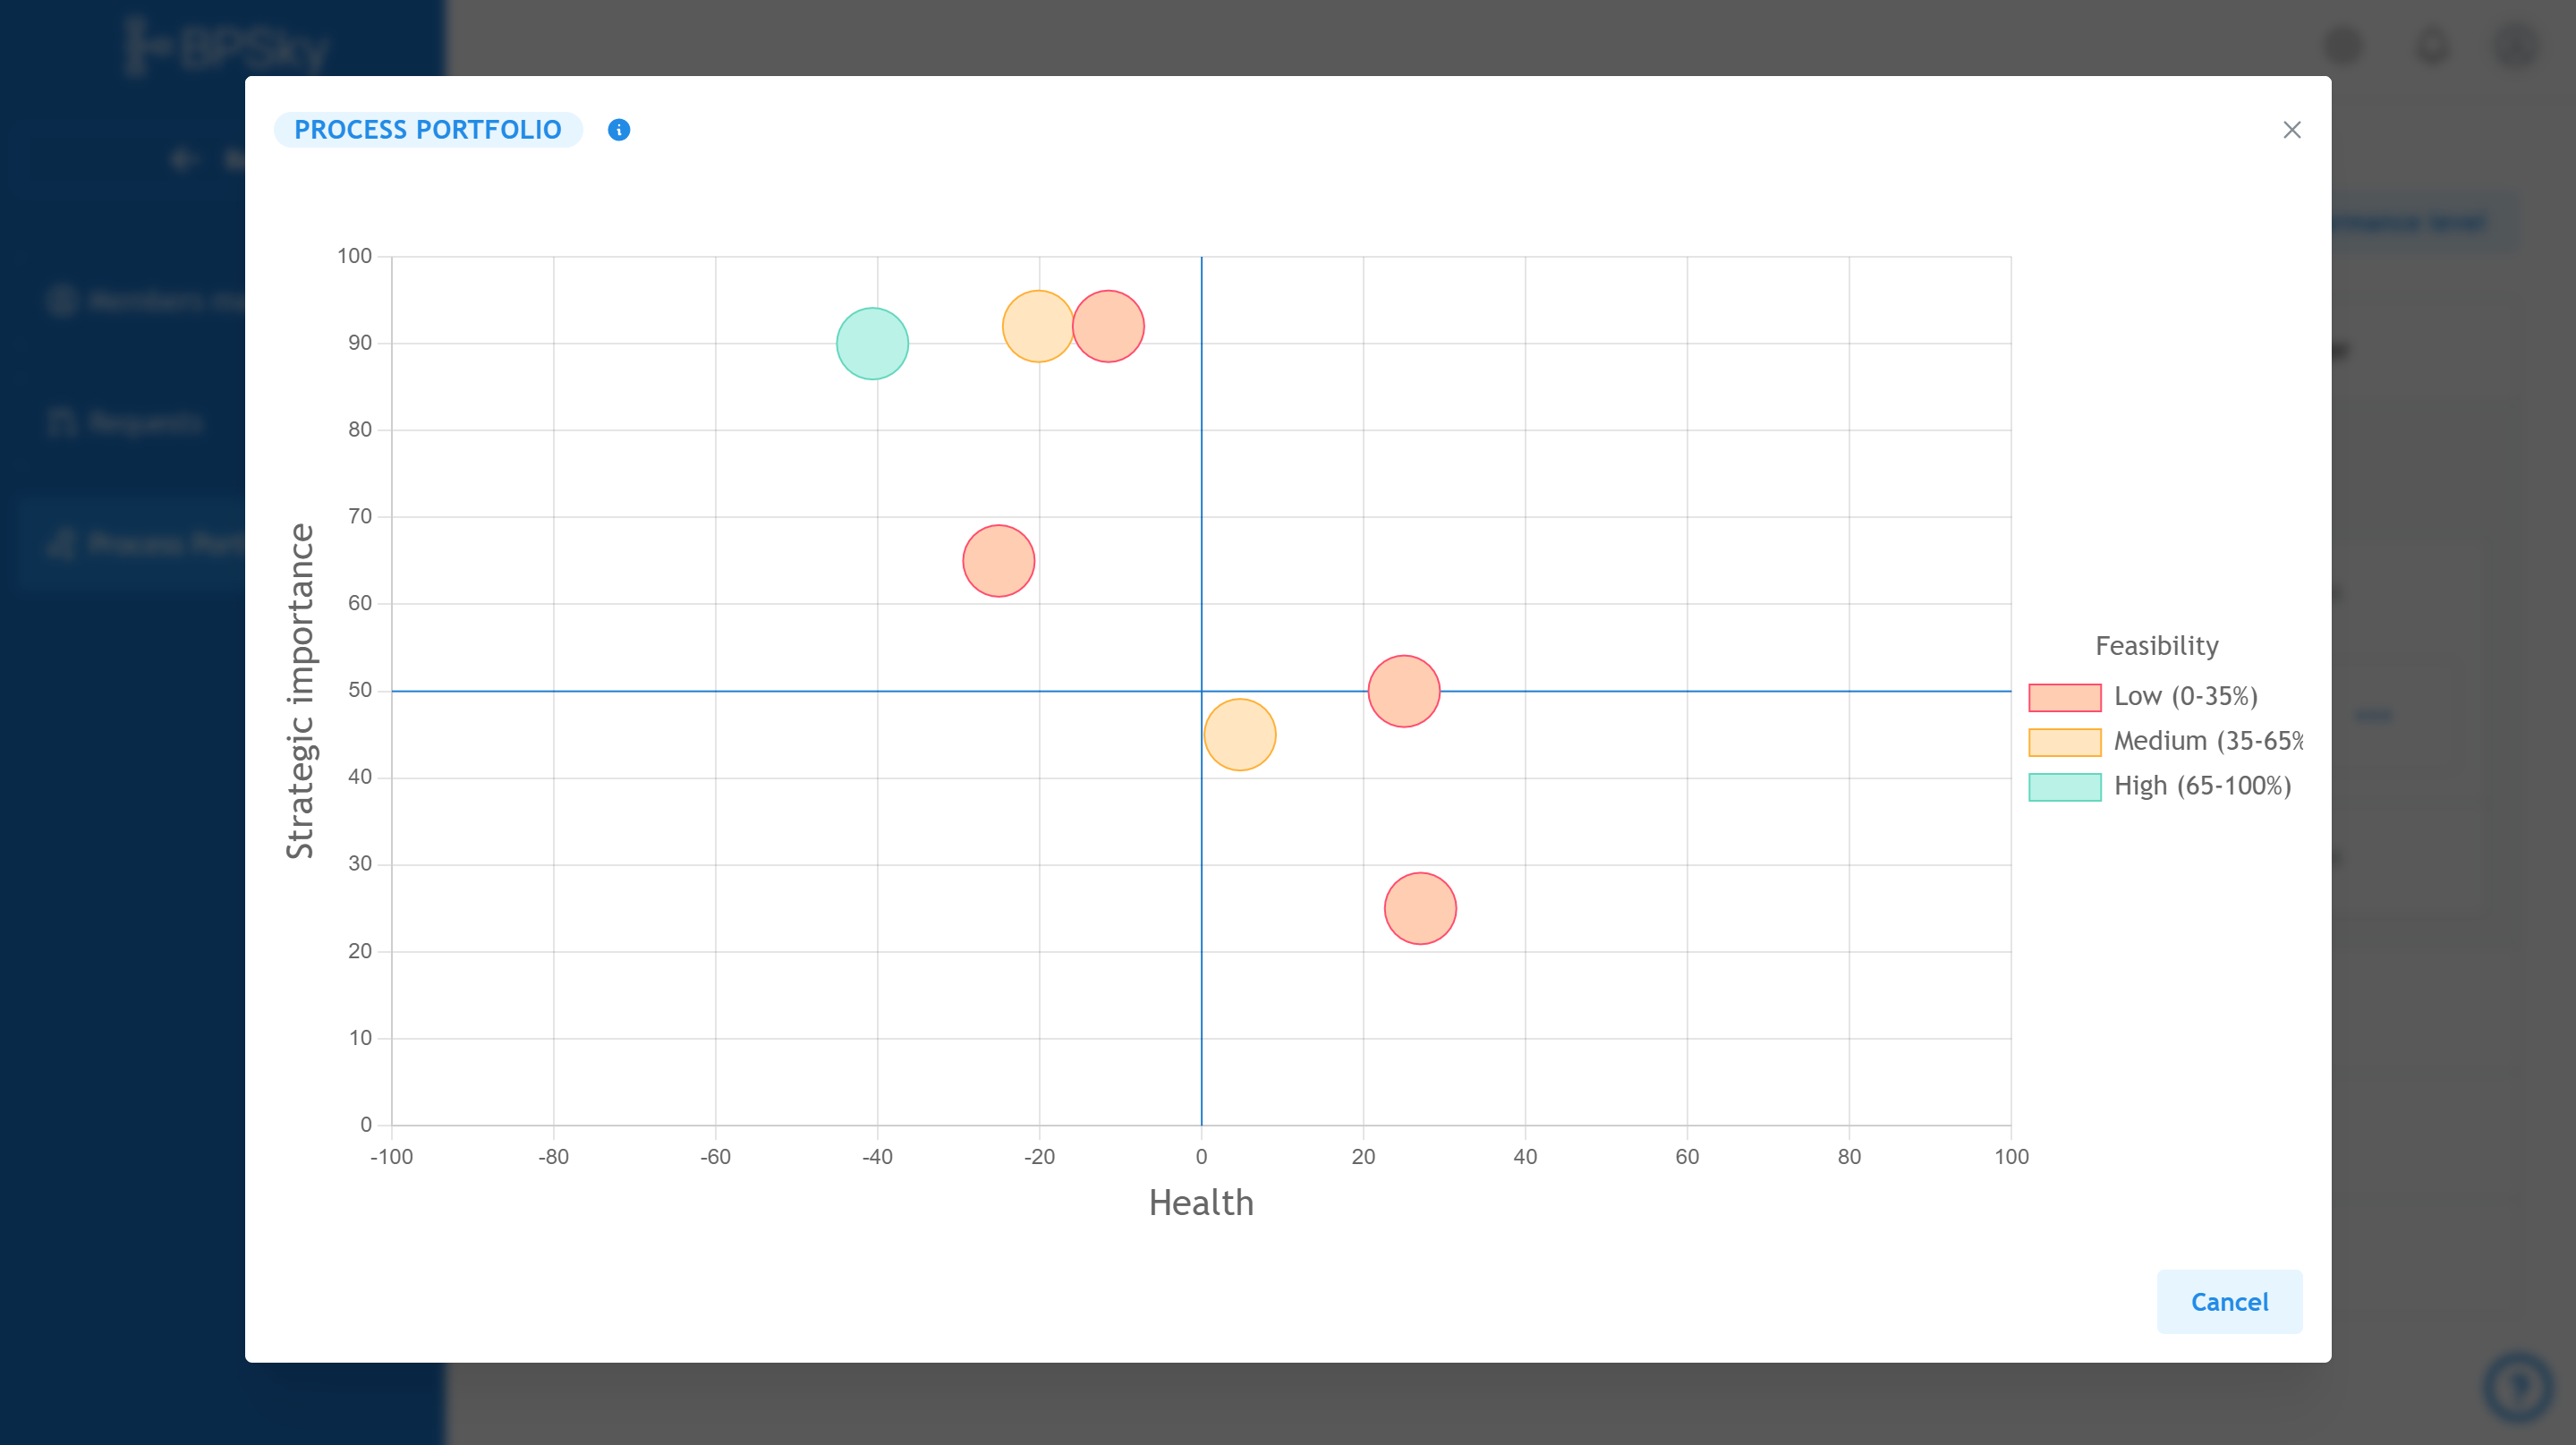
\includegraphics[ width = 0.8\linewidth]{Content/Hiện thực hệ thống/documents/Hiện thực giao diện người dùng/images/ProcessPortfolioChart.png}
    \vspace{0.5cm}
    \caption{Giao diện biểu đồ process portfolio của workspace}
    \label{fig: Giao diện biểu đồ process portfolio của workspace}
\end{figure}

Người dùng sau khi chọn nút Process portfolio thì hệ thống sẽ mở biểu đồ process portfolio của workspace. Biểu đồ này sẽ hiển thị các process version/project có trong workspace. Mỗi node sẽ hiển thị thông tin liên quan tới process version tương ứng. Màu sắc của node sẽ thể hiện tính khả thi (Feasibility) của process version. Trục tung và trục hoành sẽ lần lượt là giá trị của hiệu suất (Health) và mức độ quan trọng chiến lược (Strategic importance). Người dùng có thể di chuyển chuột qua node để xem thông tin chi tiết của process version tương ứng.

\begin{figure}[H]
    \centering
    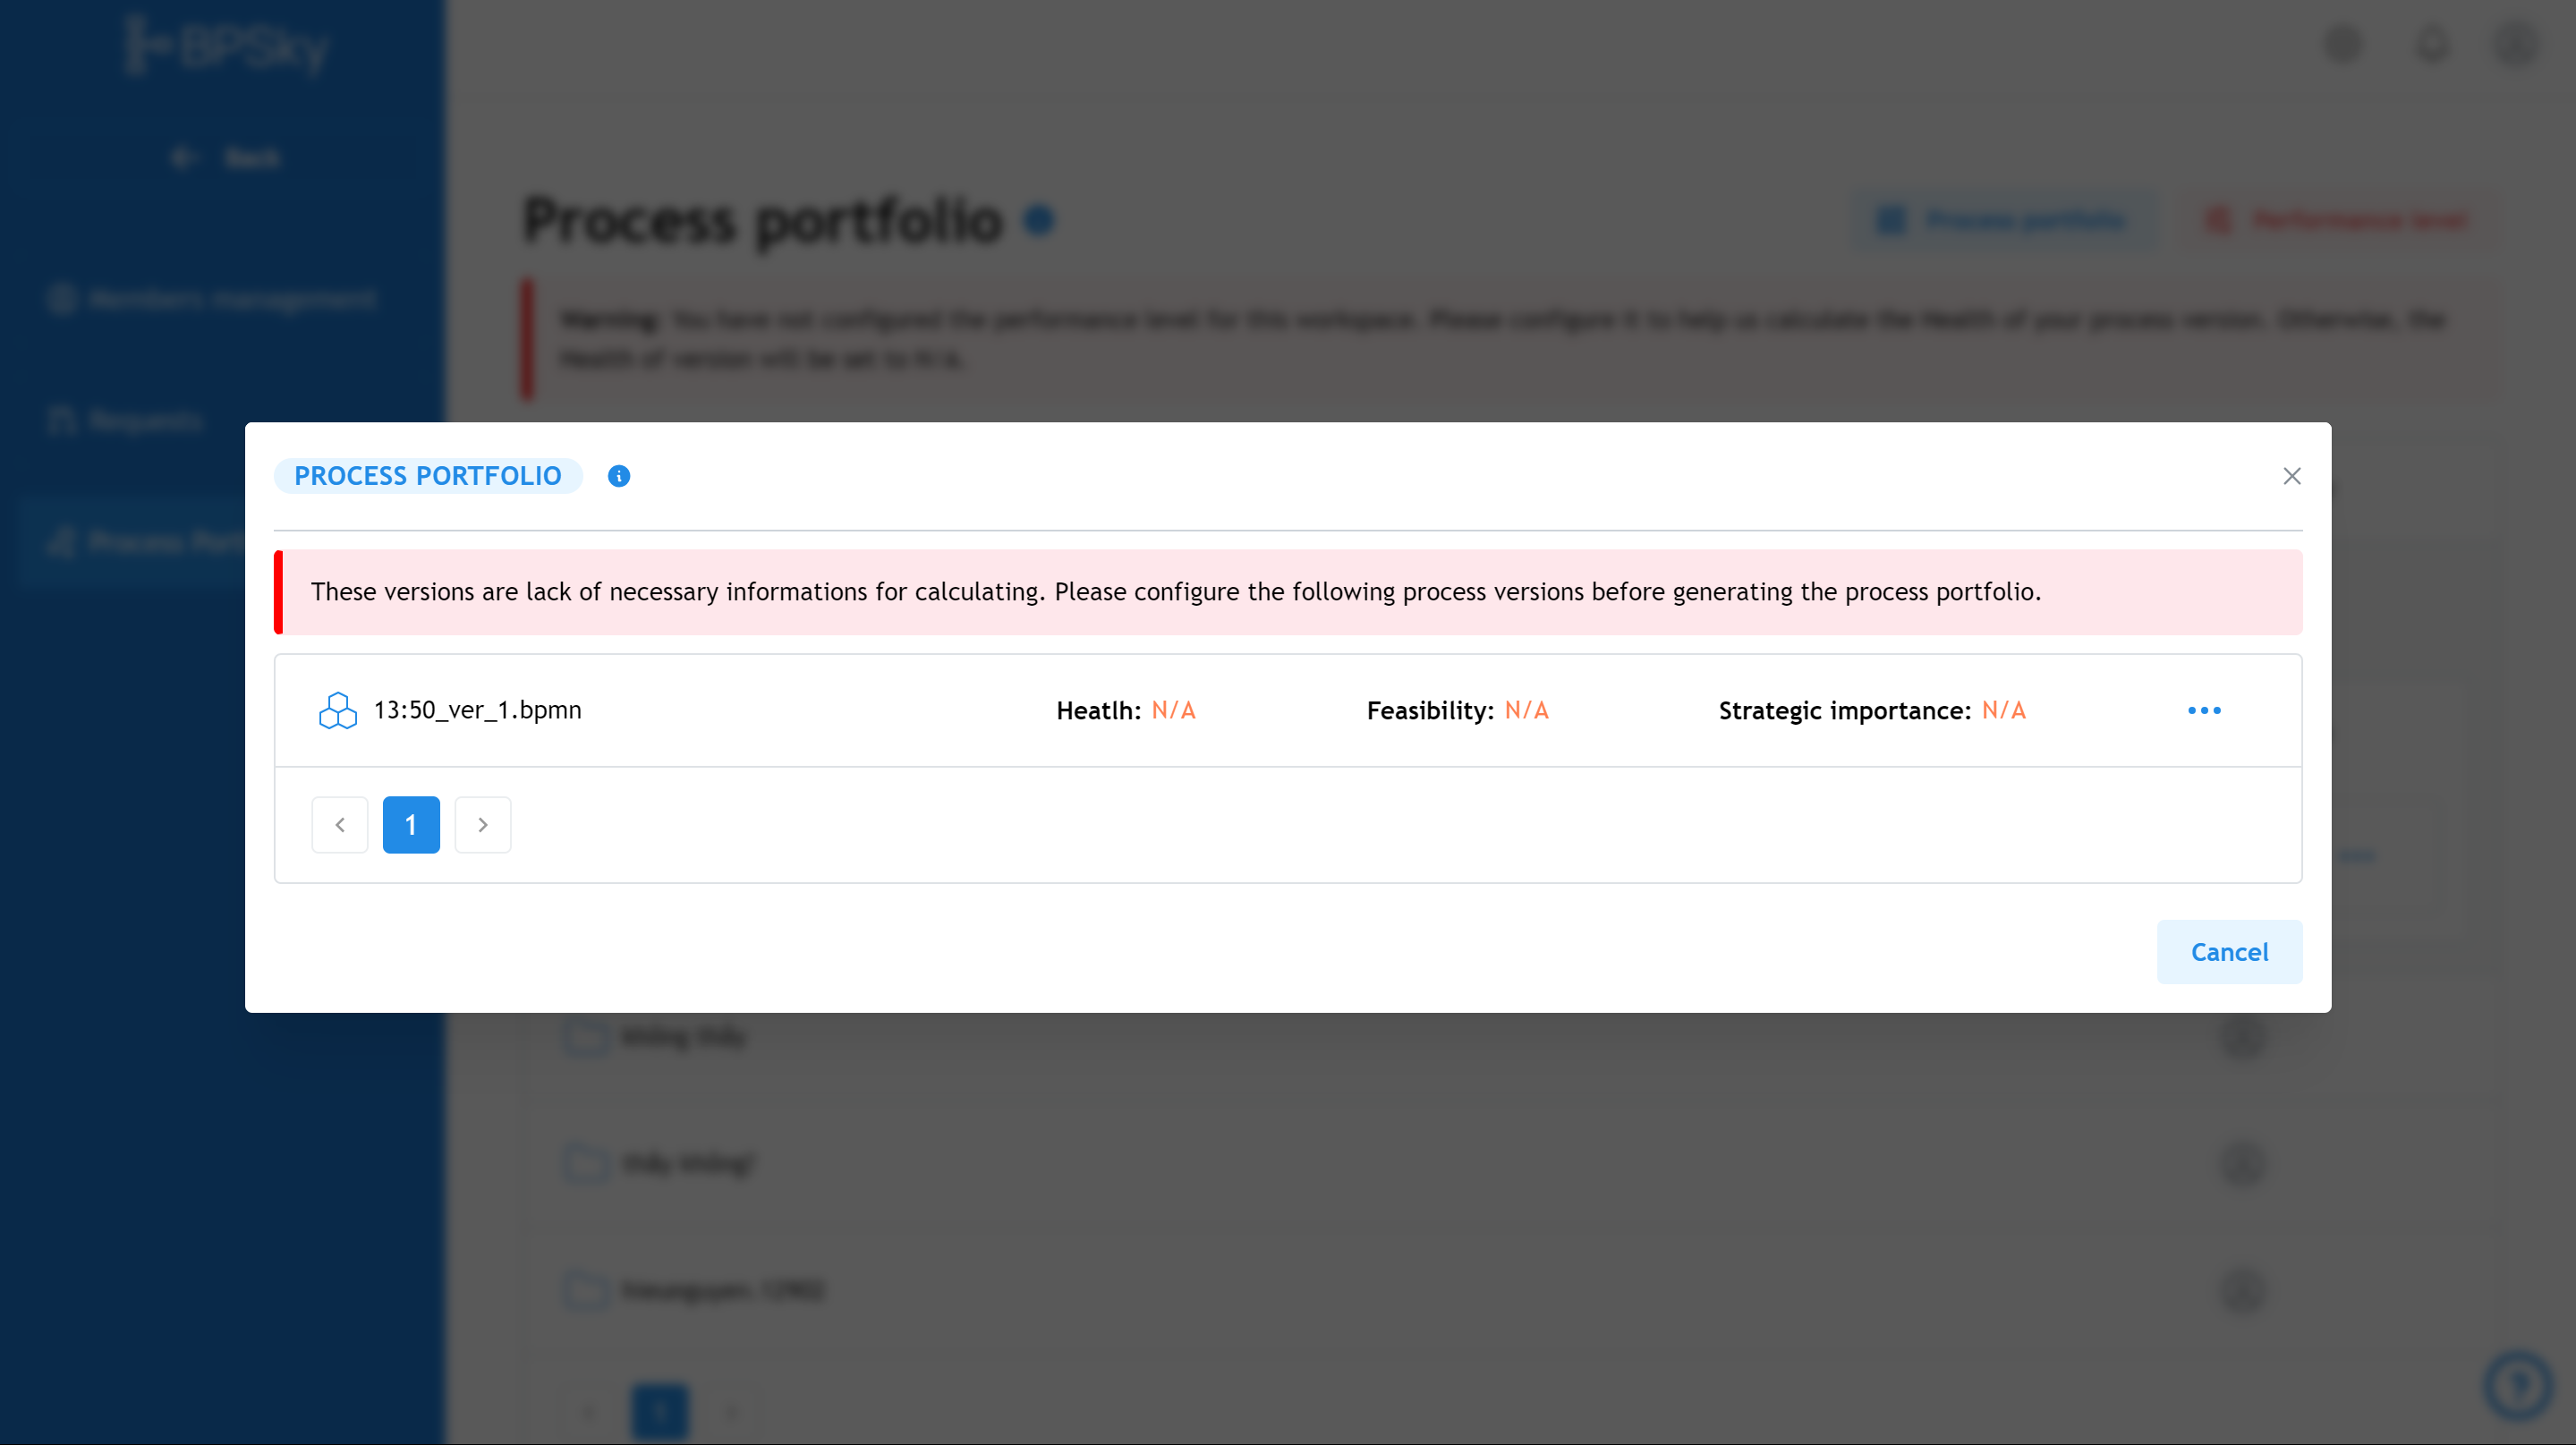
\includegraphics[ width = 0.8\linewidth]{Content/Hiện thực hệ thống/documents/Hiện thực giao diện người dùng/images/NAProcessVersion.png}
    \vspace{0.5cm}
    \caption{Giao diện hiển thị danh sách process version không có/thiếu dữ liệu}
    \label{fig: Giao diện hiển thị danh sách process version không có/thiếu dữ liệu}
\end{figure}

Nếu có tồn tại process version nào trong workspace bị thiếu dữ liệu liên quan tới hiệu suất, tính khả thi hoặc độ quan trọng chiến lược thì hệ thống sẽ hiển thị danh sách những version đó. Người dùng cần bổ sung đầy đủ thông tin thì process portfolio mới được khởi tạo thành công.